\documentclass[10pt]{beamer}

\usetheme[progressbar=frametitle]{metropolis}
\usepackage{appendixnumberbeamer}

\usepackage{booktabs}
\usepackage[scale=2]{ccicons}

\usepackage{pgfplots}
\usepgfplotslibrary{dateplot}

\usepackage{xspace}
\newcommand{\themename}{\textbf{\textsc{metropolis}}\xspace}

\usepackage[brazilian]{babel}
\usepackage[utf8]{inputenc}
\usepackage[T1]{fontenc}

\title{UNIVERSIDADE DE ITAÚNA}
\subtitle{Aprendizado de Máquina Aplicado à Valoração de Redações}
% \date{\today}
\date{19 de Junho de 2017}
\author{\textbf{Graduando:} Eugênio Cunha \\ \textbf{Orientador:} Dr. Marco Túlio Alves N Rodrigues}
\institute{{Departamento de Ciência da Computação \small} \\ {Bacharelado em Ciência da Computação \small}}
\titlegraphic{\hfill
\includegraphics[height=1.5cm]{images/uit.pdf}}

\begin{document}

\maketitle

\begin{frame}{Conteúdo dos Slides}
  \setbeamertemplate{section in toc}[sections numbered]
  \tableofcontents[hideallsubsections]
\end{frame}

\section{Introdução}

\begin{frame}[fragile]{A redação}
% O que me fez pensar no assunto?
O desenvolvimento de uma redação e uma atividade prática presente na cultura civilizada desde a invenção da escrita ~\cite{lara:1995}.

O decreto 79.298, de 24 de Fevereiro de 1977 definiu a “inclusão obrigatória da prova ou questão de redação em língua portuguesa” nos concursos e vestibulares (Art. 1 o , alínea d).

\end{frame}

\begin{frame}[fragile]{A redação no ENEM}
% O que me fez pensar no assunto?
Um bom desempenho na prova de redação no Exame Nacional de Ensino Médio - ENEM é um requisito para ser aprovado no processo seletivo de acesso a inúmeras universidades públicas ~\cite{sisu:2017} e a importantes programas de governo ~\cite{csf:2017}.

\begin{figure}[H]
\begin{center}
    
\includegraphics[scale=0.50]{images/enem_sisu_csf.png}
\end{center}
\label{fig:enem_2016}
\end{figure}

\end{frame}

\begin{frame}[fragile]{ENEM 2016}
% O que me fez pensar no assunto?
Dados da avaliação de redações do ENEM 2016 ~\cite{paq_a:2016}.

\begin{figure}[H]
\begin{center}
    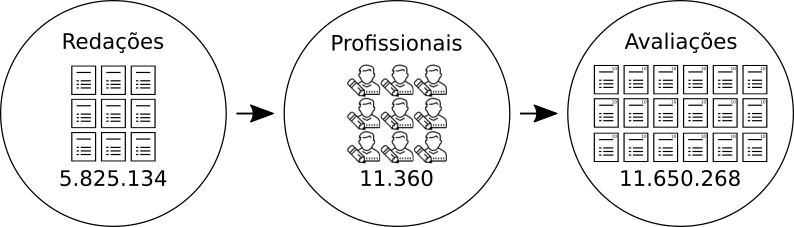
\includegraphics[scale=0.52]{images/enem_2016.png}
\end{center}
\label{fig:enem_2016}
\end{figure}

\end{frame}

\begin{frame}[fragile]{Hipótese do estudo}
% Quais as hipóteses levantadas

A hipótese deste estudo é que a classificação de uma redação por um algoritmo de Aprendizado de Máquina pode ser tão eficiênte e seguro quanto o processo de avaliação manual.

\begin{figure}[H]
\begin{center}
    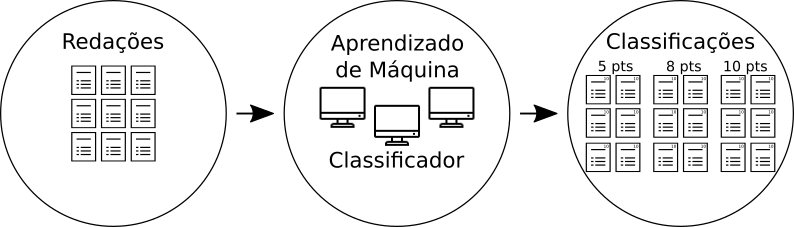
\includegraphics[scale=0.52]{images/automatic_essay_system.png}
\end{center}
\label{fig:enem_2016}
\end{figure}

\end{frame}

\section{Objetivos}

\begin{frame}[fragile]{Objetivo Geral}
Este trabalho tem como objetivo induzir um modelo de Aprendizado de Máquina a classificar as competências exigidas em um texto de redação.
\end{frame}

\begin{frame}[fragile]{Por que eu fiz a pesquisa}
Por que eu fiz a pesquisa
\end{frame}

\begin{frame}[fragile]{Quais as hipóteses levantadas}
Quais as hipóteses levantadas
\end{frame}

\section{Metodologia}

\begin{frame}[fragile]{Como será feita a pesquisa}
Como será feita a pesquisa
\end{frame}

\begin{frame}[fragile]{Métodos para obter os resultados}
Métodos para obter os resultados
\end{frame}

\begin{frame}[fragile]{Métodos de analise dos resultados}
Métodos de analise dos resultados
\end{frame}

\section{Resultados Experimentais}

\begin{frame}[fragile]{Resultados}
Resultados que eu encontrei
\end{frame}

\section{Considerações finais}

\begin{frame}[fragile]{O que foi aprendido?}
O que foi aprendido ou levantado na literatura
\end{frame}

\begin{frame}[fragile]{Próximo Passos}
Próximo Passos
\end{frame}

\appendix

\begin{frame}[fragile]{Backup slides}
  Sometimes, it is useful to add slides at the end of your presentation to
  refer to during audience questions.

  The best way to do this is to include the \verb|appendixnumberbeamer|
  package in your preamble and call \verb|\appendix| before your backup slides.

  \themename will automatically turn off slide numbering and progress bars for
  slides in the appendix.
\end{frame}

\begin{frame}[allowframebreaks]{References}

  \bibliography{demo}
  \bibliographystyle{abbrv}
\end{frame}

\end{document}